\documentclass[onecolumn, draftclsnofoot,10pt, compsoc]{IEEEtran}
\usepackage{graphicx}
\usepackage{url}
\usepackage{setspace}

\usepackage{geometry}
\geometry{textheight=9.5in, textwidth=7in}
\usepackage{hyperref}

\usepackage{listings}
\usepackage{color}

\definecolor{dkgreen}{rgb}{0,0.6,0}
\definecolor{gray}{rgb}{0.5,0.5,0.5}
\definecolor{mauve}{rgb}{0.58,0,0.82}

\lstset{frame=tb,
  language=Java,
  aboveskip=3mm,
  belowskip=3mm,
  showstringspaces=false,
  columns=flexible,
  basicstyle={\small\ttfamily},
  numbers=none,
  numberstyle=\tiny\color{gray},
  keywordstyle=\color{blue},
  commentstyle=\color{dkgreen},
  stringstyle=\color{mauve},
  breaklines=true,
  breakatwhitespace=true,
  tabsize=3
}



\def \DocType{		Final Report -Aviral Sinha
				}
			
\newcommand{\NameSigPair}[1]{\par
\makebox[2.75in][r]{#1} \hfil 	\makebox[3.25in]{\makebox[2.25in]{\hrulefill} \hfill		\makebox[.75in]{\hrulefill}}
\par\vspace{-12pt} \textit{\tiny\noindent
\makebox[2.75in]{} \hfil		\makebox[3.25in]{\makebox[2.25in][r]{Signature} \hfill	\makebox[.75in][r]{Date}}}}
% 3. If the document is not to be signed, uncomment the RENEWcommand below
\renewcommand{\NameSigPair}[1]{#1}


%%%%%%%%%%%%%%%%%%%%%%%%%%%%%%%%%%%%%%%
\begin{document}
\begin{titlepage}
    \pagenumbering{gobble}
    \begin{singlespace}
    	%\includegraphics[height=4cm]{coe_v_spot1}
        \hfill 
        \par\vspace{.2in}
        \centering
        \scshape{
            {\large\today}\par
			{\large CS463 Spring 2018}\par
			{\large Group 68}\par
            \vspace{2.5in}
            \textbf{\Huge{Final Report Aviral Sinha}\par
			\textbf{\Huge{HedgeServ: Investment Performance Mobile App}}\par
            \vspace{2.5in}
            {\large Prepared by }\par
            \vspace{5pt}
            {\Large
                \NameSigPair{Aviral Sinha}\par

            }
            \vspace{20pt}
        }
      
    \end{singlespace}
\end{titlepage}
\newpage
\pagenumbering{arabic}

\section{Tech Review (Original)} 


\subsection{1. Data Services}

\subsubsection{1.1 Overview}
My role in this project is that since i have the most finance knowledge out of my group members I will be handling what data we will be getting, how it will be visualized, and then properly developing it on a platform that gives us the highest chance of success. The data services we choose to use will largely depend on the portfolio that our users will have. Since it will contain mostly stocks and options we limit ourselves to public companies on the NYSE and make sure our data output is as accurate as possible.For this part of the piece we will be discussing the web services aspect of our application. With our project we will be using established constraints and consistently pulling data from financial instruments like the US Dollar, stocks, options, and other types of securities. With mass amounts of data being needed for our user to access this on their mobile phone we will be needing to pull from external web services. Since the financial services industry is already established and has various enterprise software, for this project we have been limited to using only free third party software outside of the ones given to us by HedgeServ. Our application will be pulling real time data from publicly traded companies and in the case of our app it will be showing investments that the user has in their portfolio. Based on our research and input from the client we have three possible choices: Quandl, Bloomberg, and Intrinio.


\subsubsection{1.2 Criteria}
For this piece the main criteria we will be looking at if the datasets we use are not only free but also cover all the various investments we will be needing to display that would be catered to the users specific portfolio. There are many possible options available that all have their own benefits. Luckily the plethora of options allows various applications to be used by different developers who are each wanting something different. When choosing a platform to use data we mainly looked at whether or not the service had an option for free use and whether or not the platform would be able to support the financial data we wanted to be looking which in this case is stocks and stock options. If it didn’t meet any of those requirements then it wouldn’t be chosen. We narrowed down our search to Bloomberg, Quandl, and Intrinio through suggestions from our client. Bloomberg is the industry leader in financial data so we obviously had to include it in consideration. Quandl and Intrinio on the other hand were suggested by our client as possible resources and after looking into what is offered the services the two provide greatly rival what Bloomberg does. 


\subsection{1.3 Potential Choices}

\subsubsection{1.3.1 Quandl}
Quandl delivers financial, economic, and alternative data to a quarter of a million people around the world and by having very large datasets at their disposal they claim to have an unrivaled size. We would be accessing their data through an API that can be used in R, Python, Matlab, Maple, and Stata.[1] For our project we would implement the API into a python environment. There’s also an option to use an add-on that lets Excel access various pricing information. The benefit with Quandl is that in addition to the usual library of paid datasets they have a vast array of free ones that have all the information we need to properly develop our mobile application. Quandl sources its data from the UN, World Bank, various other central banks, providers like the CLS Group, Zacks and ICE, and then it also gets its alternative data from Dun \& Bradstreet.[1] Since its launch 6 years ago it has quickly grown into a major player in the financial data sector. One of the main reasons for their success is partly due to their sales of alternative data sets, which aren’t typically offered by traditional sources. By finding, evaluating, and the productizing undiscovered data they are able to enhance the trading strategies of their customers. Similar to Apple’s App Store Quandl has a marketplace where it clearly displays all the various sets with the clear distinction between what is free and what requires their premium subscription. 

\subsubsection{1.3.2 Bloomberg}
The next choice we have is Bloomberg, more specifically their Bloomberg Terminal. This is the industry leader in monitoring and analyzing real time financial market data and allows it to be used as a platform for electronic trading. While the main Bloomberg Terminal product used by most firms on Wall Street costs \$20,000 per user, they have recently announced an Open API that will allow third party applications to access data and create independent calculations from the terminal interface. [2] With this API our application would be able to access current, historial, and reference market data and build formulas for trading decisions. Originally the API was only offered for Excel but now it is available for most major programming languages, for our project since we will be using .NET and python it’s very beneficial that Bloomberg is supported on these platforms. [2]

\subsubsection{1.3.3 Intrinio}
The final choice we will look at is Intrinio, they market themselves as able to help investors save money, by cutting time down on data collection, data entry, and data analysis the production of an analyst rapidly decreases as their tasks become more tedious than meaningful.[3] They make the data easy to access for developers and allow for full creativity and customization. The datasets they offer include, FDIC bank data, real time IEX stock prices, US 10Q/10K data and insider transactions.[3] By having a vast library data sets it makes investors easily conduct research and make strategic decisions. The only problem with this option is that it requires a fee for the subscription. 


\subsubsection{1.4 Discussion}
The three choices presented above essentially all offer the same product, but each one has their own pros and cons. With Quandl we essentially have all the datasets we will need in addition to any alternative data that may possibly need in the future all for free as the paid datasets are very particular in application and are required for our project. Bloomberg surprised us in that they now have a free and open API but the infrastructure and datasets provided by Bloomberg are best used with a full Bloomberg environment rather than in a completely different ecosystem like the one we are developing, and while using Bloomberg would be the most ideal it's not feasible to spend over \$20000 on of their terminal platforms. Intrinio is definitely the latest entry in this industry of financial data and while what they offer can prove great to use to us, they are also requiring a subscription fee and with it being relatively new we would definitely be running into a lot of problems with a proper implementation of their data. 

\subsubsection{1.5 Conclusion}
In conclusion we decided to choose Quandl because of its ability to provide various types of data that will be able to fulfill the requirements we set and properly allow a user to access the various types of investments they want to look at. With HedgeServ mainly working with Hedge Funds we need to be able to see alternative data as well as they will play a factor into a user’s portfolio value and by implementing various types of data we can assure high returns. It's also beneficial that we can use most of Quandl services for free which lowers the overall cost of production. 



\subsection{2. Data Visualization}

\subsubsection{2.1 Overview}
In this piece we will be looking at the various solutions to how we can visualize data within our application. The user’s portfolio will vary in investments and with data easily shown through pie charts or graphs it allows for the user to glance at it quickly and make decisions. The visualizations will also help serve historical investment prices and show various other variables related to that security. The main purpose of this is to help make the app look clean and simple but also able to convey its data very easily. The inspiration for this is from investment applications like Coinbase and Robinhood which both use visualization to make it easier for their user base to look at investments and make decisions. The three choices for this are Google Charts, Keen IO, and Drupal. 

\subsubsection{2.2 Criteria}
The main criteria for this will be similar to the last piece in that we will be wanting our service to be free and also have the ability to handle and properly display our various types of data. We will also need this tool to be easily integrated with the rest of our application, that means that it needs to work with the mobile platform we are developing on, easily display on our front end as well as pull in data from our backend and then access the various data sets we are using from Quandl.  We brought choices down to these three based on research as well as consultation from our client. 

\subsubsection{2.3 Potential Choices}

\subsubsection{2.3.1 Google Charts}
Google Charts was the first one that we thought of because of how prevalent it is in freelance data visualization work and has many available resources and code examples which will help make our job easier and we can properly display a user’s portfolio as well as trends and graphs for investments they are interested in adding. With Google we will also get access to a vast library of suites with their Charts product line where we can implement various ways of displaying data. A benefit of using this choice is that we will be able to easily port this data to be easily available on both android and iOS which saves us the trouble of optimizing the data. A drawback is that we will be limited to using javascript to create this API which means that we will be making both our frontend and backend a bit more complicated.[4]

\subsubsection{2.3.2 Keen IO}
The next option is Keen IO which will allow us to easily collect data, enrich it for our needs, and then send it to a destination. With this we will also get full customization over the stack and have the ability to make all the decisions when it comes to choosing which data is relevant. Like the rest of the options they also guarantee low operation and delivery risk which means that our data pipeline won’t be fault tolerant.[5] Keen IO’s ability to access any time of data from any source benefits not only our required goals but also help support our stretch goal of bringing in related news into a data stream, by pulling in data from articles that have information related to an investment this allows us to easily compile it and put it all together for the user to not only see how a stock does in their own portfolio but also see what the media and other analysts are saying. The major drawback though is that we will have to keep our data stream below \$20 worth of usage if we want the service to be free.[5] The moment we go over then we will be charged by Keen IO. 

\subsubsubsection{2.3.3 Drupal Visualization API}
The last option we will be looking at is Drupal’s Visualization API, this will be the simplest option for us because it easily takes a data array and then makes a chart out of it. It also uses some of the features from the Google Visualization API which means that we will be getting access to their vast resources and libraries in a more controlled environment that won’t be too overwhelming for us.[6] Since this API is open source we also get the benefit of it being free and able to get help from Drupal’s huge open source environment. One of the few drawbacks of this though is that it may not be fully compatible with our project’s framework but we would definitely look into a way of getting around this. [6]

\subsection{2.4 Discussion}
The three choices above all give us various options in how we want to present our data. Both Drupal and Google are essentially the same product with just a slight variation in what they offer to us as a client in contrast to Keen IO which is vastly different in what it offers and truly allow us to present all the data we need to show. Like I explained in the first piece having the ability to look at alternative investments will greatly benefit our users because our investments can vary in scale and type, using tools that can accommodate this will be crucial to the success of our app. Keen IO’s limitation on data usage for a free membership is what really taints its ability to be our primary tool for data visualization, if anything we could use it as a supplementary tool in addition to our main one for showing data that can’t shown by our primary option. 

\subsection{2.5 Conclusion}
In conclusion we will be using Google Charts visualization tool because of its vast array of libraries, resources, and tools that will make our job of displaying portfolio information in a very beautiful and clean manner. Like I mentioned in the discussion if required we will implement some of Keen IO’s tool into our visualizations if Google can’t properly display all the data we need. Like the previous piece our choice in what technology we use comes down to its functionality and cost (or lack thereof) which plays a heavy  hand in our decision making process. Luckily this helps us narrow down the technologies we need very easily as there are a plethora of possible options for how we can display data. 


\subsection{3. Mobile Application Development tools }

\subsubsection{3.1 Overview}
In this section I will be discussing the different mobile application development tools we can use to properly build this application. There are three ways we can go about the development of an application that will be primarily used on iOS and Android. The first option is Xamarin which is a single tech stack and single codebase using C\# and .NET, another option would be to use a native platform with different tech stacks for each platform, and then finally we could use a Hybrid method like Apache Cordova which has one tech stack and one codebase but its in javascript, html5, or CSS.

\subsubsection{3.2 Criteria}
I will be measuring these three choices through a few different criteria. I will be looking at whether they have code sharing, UI/UX customization, how good is their performance, their hardware capabilities, and how long it takes for a product developed on the platform to go to market. Essentially these criterias will compare the three different development methodologies that I described in the overview and allow us to decide on whether or not we want to go with something industry standard or is it possible to achieve better results with an alternative that may have not been considered. 

\subsubsection{3.3 Potential Choices}

\subsubsection{3.3.1 Xamarin}
The first option that we'll look at is Xamarin, this was suggested by HedgeServ as the best option for us to properly and more importantly easily develop our application without running into various problems that could delay a release. Though its relatively new its used by millions. Its an interesting option because it uses C\# and native libraries that are wrapped in the .Net layer to allow cross platform development. Not only is it cross platform but it also allows for platform specific UI code layer which makes a cross platform application look native on any device.[7]

\subsubsection{3.3.2 Native Platform Development}
The next option would be to develop it natively for each platform. This would require us to separetely develop each version. For example for our android version we would develop it in Java and then our iOS version would be built using either objective C or swift.[7] This would definetely increase the level of performance as it will be the purest way of development. The application will also feel most at home on their respective platforms but at the cost of a slower time to market.

\subsubsection{3.3.3 Apache Cordova}
The final option we are looking at is the use of a hybrid platform like Apache Cordova. This option would be a web based technology that wouldn't really be native but offer an easy alternative for us to quickly get working code onto a mobile platform. One of the popular hybrid options would be Apache Cordova uses CSS, HTML, and javascript instead of platform specific APIs. It then wraps up the code depending on the device. Apache Cordova is unique because it is neither a truly native mobile application nor web based. Cordova is also used as the base for many other web based development platforms like Telerik, Intel XDK, Ionic, and visual studio. Having all of these different options allows for Cordova to have a rich ecosytem of support for when any major development problems occur. [8]

\subsubsection{3.4 Discussion}
Each of the three options above all of have their pros and cons. Xamarin makes use of a single tech stack with a single codebase using C\# and .NET frameworks. It also allows up to 96\% code sharing and the UI can be fully customizable with each device platform having a unique look.[7] The performance is very good and almost as good as a native application. With Xamarin we also get the use of platform specific APIs and linking of native libraries which make the hardware capabilities great. Xamarin also allows for a somewhat quick time to market compared to a native application.[7] In comparison to Xamarin and Hybrid options using a native platform will have different tech stacks for each platform with different code bases and each platform having a specific UI made for it. On the other hand though, this level of detail allows for excellent performance and a high level of hardware capabilties because of it has support right out of the box. The main problem is that the time to market will definetely take a lot longer because we would have to develop the iOS and Android app separately on different platforms which increase the time considerably, but in return we would get the highest quality product.[7] The last option discussed was using a hybrid platform development tool, more specifically the use of something like Apache Cordova, this would have one tech stack with a single codebase in either javascript, html5, or CSS and have a 100\% codesharing.[8] Since this would be a lot more limited in scope it would have a common UI for all the platforms with very little customization abilities and performance would be relatively bad. The hardware capabiltiies will also be limited because it can be accessed through third party APIs and plugins but there is a high level of risk because of the poor quality and unreliability of the tools. Since developing on a hybrid platform is relatively easy, these solutions are the fastest to market because of the single code and little to no customization involved. A hybrid solution is best used for early development prototyping and proof of concept projects that want to display what the final product will look at the end of development. [7]

\subsubsection{3.5 Conclusion}
In the end we are going to be used Xamarin because of its numerous benefits as well as being recommended by our client. Its use of one technology stack to code for all platforms, its close to native performance that beats all of its competitors. It also has very native use expierences that are basically flawless. Its ability to work with various APIs eliminates all potential risks that we would have faced with compatibility. Another benefit of Xamarin not mentioned above is that it is open source technology with a strong corporate support and allows for application maintenance to be simple and easy. Finally we found the ecosystem developed by Xamarin to be very ideal in that it has its own IDE, platform, testing, distribution and analytics which make our development process very streamlined and efficient. 




	
\subsection{Works Cited}

[1] \textit{“New Data Provider Quandl Moves Toward Alternative Data • Integrity Research,” Integrity Research. [Online].} Available: \url{https://www.integrity-research.com/new-data-provider-quandl/.} [Accessed: 20-Nov-2017].

[2] Z. M. Seward, \textit{“This is how much a Bloomberg terminal costs,” Quartz, 15-May-2013. [Online].} Available: \url{https://qz.com/84961/this-is-how-much-a-bloomberg-terminal-costs/.} [Accessed: 21-Nov-2017].

[3] \textit{“Intrinio - Female Led Start-Up Attracts Top Institutional Investors,” ValueWalk, 24-Oct-2017. [Online].} Available: \url{http://www.valuewalk.com/2017/10/intrinio/.} [Accessed: 21-Nov-2017].

[4] \textit{“Using Google Charts  |  Charts  |  Google Developers,” Google. [Online].} Available: \url{https://developers.google.com/chart/interactive/docs/.} [Accessed: 21-Nov-2017].

[5] A. Ha, \textit{“Custom Analytics Startup Keen IO Raises \$11.3M Round From Sequoia And Others,” TechCrunch, 01-Jul-2014. [Online].} Available: \url{https://techcrunch.com/2014/07/01/keen-io-series-a-sequoia/.} [Accessed: 21-Nov-2017].

[6] \textit{“Data Visualization API,” Drupal.org, 01-Dec-2014.} [Online]. Available: \url{https://www.drupal.org/project/data_visualization.} [Accessed: 21-Nov-2017].

[7] \textit{“The Good and The Bad of Xamarin Mobile Development,” AltexSoft. [Online].} Available: \url{https://www.altexsoft.com/blog/mobile/the-good-and-the-bad-of-xamarin-mobile-development/.} [Accessed: 20-Nov-2017].

[8] \textit{“Overview,” Architectural overview of Cordova platform - Apache Cordova. [Online].} Available: \url{https://cordova.apache.org/docs/en/latest/guide/overview/index.html.} [Accessed: 21-Nov-2017].







\section{Weekly Blog Posts} 

\subsection{Fall 2017} 
 \subsection{Week 1}
    During week 1, we looked over and gave our first 3 choices for projects to Kevin. We all chose this project as our first choice. 
    
    \subsection{Week 2}
    This week, we had our first meeting with Brice Lemke. We introduced ourselves and presented him with our backgrounds. He gave us a very general overview of what the application would entail which was already basically within the project description. Additionally, we set up a weekly meeting time. We also set up a means of communication through an IM app called Slack.
    
    \subsection{Week 3}
    This week we received our first email from our TA, Andrew. We set up a weekly meeting with him. We also reviewed the rough drafts of our problem statement in class.
    
    
    \subsection{Week 4}
    This week we submitted and finalized our problem statement with our client. We further revised and understood more nuance about the expectations and requirements of the project.

    
    \subsection{Week 5}
       This week we submitted our rough draft for our requirements document, we also met with our TA for the first time this week, Andrew, after it requiring a period of time do agree on a time slot with him 
    
    \subsection{Week 6}
        This week we discovered and we had it shared with us that our client will no longer be at HedgeServ. We were supposed to supply our client with our requirements document by Friday, and he didn't respond on any of the days we reached out. We had an email sent to us by one of his coworkers stating that he was no longer working there and we would have to begin working with someone else. 
 
        We submitted our "final" requirements document unsigned to our TA, and will need to have it signed at a later date 
        
        We have plans to meet at our new time with our new client on Wednesdays at 12-1. We will bring him/her up to speed as soon as possible in order to keep the project moving 
            
    
    \subsection{Week 7}
        This week we had our first meeting with our new client, Edison Tsai, and Ronald Olshausen. Ronald's vision for our project differed greatly from Brice's so moving forward we are going to have to more or less go back to the drawing board and start from scratch on our requirements document, 
 
        We updated Andrew, Kirsten, and Kevin all individually and informed them of the situation. Going forward we have loose deadlines on some of the documents, and can request extensions if needed. 
 
        This coming week we plan on redoing our requirements document and submitting that to Edison/Ronald for review. 
    
    \subsection{Week 8}
        This week we met with our new client for the second time and got a much better idea of what their vision is for the new project. It was very reassuring, and we received enough information to fully revise and resubmit our requirements document to our client for approval. Next week, we have our tech review due, but Kirsten gave us an extension. I plan on submitting the tech review after the break. 

            
    \subsection{Week 9}
        This week we submitted our new requirements document and discussed it with our client in our weekly meeting. We were granted tech review extensions by Kirsten and had a deadline for after thanksgiving weekend. Not much was done or shared this week, and everyone in our group is going different places for thanksgiving and going to write and submit the tech review this weekend/week. 

            
            
    \subsection{Week 10}
        This week,We got feedback on our tech reviews so it could be implemented properly in the design doc. Additionally, we began discussing the design document and received an extension on that until next Friday 12/8. We also discussed our meetings over winter break with our client, and we agreed that there wasn't a need to meet during our time off and we would reconvene in January. We also got feedback from Andrew about our requirements document, and he shared with us that our biggest flaw was missing IEEE standards, and that we need to make sure to meet them when he grades the design document. 
        
        
\subsection{Winter 2018}
    \subsection{Week 1}
    We talked to each other about what times work for us for both client meeting times and TA meeting times. Began to look at what steps need to be taken for tackling the app development. Kevin showed us KEC 2098 lab access and went over the term's work schedule. 
    
    \subsection{Week 2}
    Met with Ron and Edison and went over what Xamarin tools were needed. Began to split up work. Alpha due in 4 weeks and still need to get a signature on the design doc from Ron and Edison. No response from Andrew regarding TA meeting times, we brought the issue up to Kevin and Kirsten
    
    \subsection{Week 3} 
    Still no response from Andrew regarding TA meeting times. We continued work with ios/android development as well as database development.
    
    \subsection{Week 4}
    We continued development, I began to look at how to implement our APIs into the project as that would take a large amount of time. We discussed what need to be done for the poster as well as other logistics in class and still had no contact with Andrew. We plan on finishing the Alpha by the end of next week.
    
    \subsection{Week 5}
    Back end and Front end work continued but this time with the use of Xamarin forms so we would have a common codebase for both apps. I started the implementation of the Quandl API. We finally met with Andrew and discussed our work and any concerns. During our client meeting we mainly dealt with the problems that have been occuring with the database and REST APIs. Once the database is set up then the API and UI will be the main priorities. I started writing an API wrapper in C# for Quandl.
    
    \subsection{Week 6}
    We had a group meeting where we discussed work that needed to be finished by the progress report at the end of this week. We also had a TA meeting where we discussed what would be coming up next. 
    
    \subsection{Week 7} 
    This week I was facing a bunch of problems with visual studio which heavily slowed down my progress this week. Since visual studio had only recently been released on Mac I was running into a lot of issues with the environment as a whole. Debugging and fixing this took a majority of my time. 
    
    \subsection{Week 8}
    I was able to properly get a REST API to function in successfuly parsing data. Got help from Andrew regarding a problem in my code because it was an issue out of both my groupmate's scope and no online resources were helpful. We arranged a demo next week with our client. Also during our small class session we talked to the other HedgeServ group who recommended using Last10k and Alpha Vantage over Quandl because those are completely free while Quandl requires a premium membership for specific data. I decided to go back to the drawing board and start with the implementation of those APIs as they would be more useful in our app. 
    
    \subsection{Week 9} 
    Continued transition into Alpha Vantage. They have a whole Nuget package available within visual studio which made it easy to access most of their data. I was able to get the time series data for specific stocks to display over the course of a few years. We showed what we had to the clients and decided to update most data on the server side each day. Dropped stock options as it wasn't supported by any open source platforms properly. Started looking at Last10k as well so we could get data populated for the  details of each stock.
    
    \subsection{Week 10} 
    With Last10k I was able to get successful parsing of a few of the key ratios needed as recommended by the client. So far I had gotten the Return on Equity, Return on Assets, EBITDA, and Inventory Turnover. During our client meeting we went over some UI and Database issues and got clarification of some of the business logic. For the sake of simplicity we will not be including ETFs (Exchange Traded Funds) and making the core database of stocks to be the Dow Jones 30 Index. The purpose of this decision is that the index holds a bunch of major US companies whose performance can directly impact the economy so by showing companies in different industries we can create various portfolios that show diversity. I handed off Alpha Vantage to Tyler so he can begin the portfolio level calculations that consist of R squared, Alpha, and overall returns. I have now set up most of the calculations regarding Last10k. They will consist of  Inventory Turnover, Return on Assets, Return on Equity, EBITDA, Asset Turnover, Total Assets, Receivables Turnover, Net Income, Earnings Per Share, Interest Coverage, Total Current Assets, Tax Rate, Free Cash Flow, and Revenue. All of these ratios come from 3 major documents: Balance Sheet, Cash Flow, and the Income Statement. We also began writing our winter progress report. 
    
\subsection{Spring 2018} 
    \subsection{Week 1} 
    Finished most of beta development. Still need to finish some work regarding Last10k as well as new client issues have risen with lack of contact. We sent follow up emails with our availability but have gotten no response.

    \subsection{Week 2} 
    Heard back from Edison who explained that due to company restructuring they won't be as involved in the project anymore. We began talks with Kirsten, Kevin, and Andrew on how to do deal with this situation. Also put in requests for equipment needed for expo. 

    \subsection{Week 3}
    Continuing development of Asset Details. After having it successfully parsed through the API, I had the data sent into our ENGR database where our application would then call it for each stock. 

    \subsection{Week 4} 
    Got asset details to show up on the mobile application. Beginning to fix any problems with the specific stock details.

    \subsection{Week 5} 
    Fixed formatting of the page. Double checking data in database to see if its being parsed correctly.
    
    \subsection{Week 6}
    Preparing for expo by debugging any other problems in the application. 
    
    \subsection{Week 7}
    Issue with stocks not in the Dow Jones showing up in the database for specific portfolios. We fixed a problem where it was crashing when clicking the stock. Instead it would return a null value to signify that we don't support that company. Also began preparing our pitches and presentation for Expo.
    
    \subsection{Week 8} 
    Presented at Expo. 
    
    \subsection{Week 9}
    Discussed what was needed for the final report in class.
    
    \subsection{Week 10} 
    Began working on the final progress report and started compiling all the documents together. 
    
    
\section{Conclusion and Reflections} 
    \subsection{What technical information did you learn?} 
    I learned a lot about software and mobile development, agile development, version control, REST APIs, C# and SQL.

    
    \subsection{What non-technical information did you learn?} 
    I learned a lot about combining finance with software development. Portfolio and Asset level calculations being taken from their native excel environment and adapting them into our environment for the application.

    
    \subsection{What have you learned about project work?} 
    I learned a lot about working with various other parties both in the immediate development group as well as with a boss(client) and other significant individuals(TA). We were able to delegate work properly and it was up to us to set deadlines and make progress and complete the project by the time it was expo. 
    
    \subsection{What have you learned about project management?} 
    My skills in project management only improved with capstone. I learned how to manage tasks that I had weekly as well as delegate tasks. I learned how to properly use tools like github and slack  to make sure all of our work was able to stay on track and we could see each others progress.
    
    \subsection{What have you learned about working in teams?}
    Working as a team I learned a lot about how dynamics can be affected over the course of a year and how we have to constantly be planning ahead. Our issues with the client through the year caused a lot of distress as they kept on disappearing so we had to constantly communicate among each other so the project could progress and be completed 
    
    \subsection{If you could do it all over, what would you do differently?}
    If we could do it differently then I would definitely have started development either fall term or during winter break because while 10 solid weeks of development is enough time having extra time in the end to debug any issues would have been very helpful. I also should have done more research in what APIs we were using because none of the ones we chose in fall term seemed viable for our final product. Our client recommended Quandl but the data needed from the service was only available to premium members and our visualization tool was replaced with Xamarin’s own charts tool which we learned about as we understood Xamarin even more. 

\section{Final Poster}

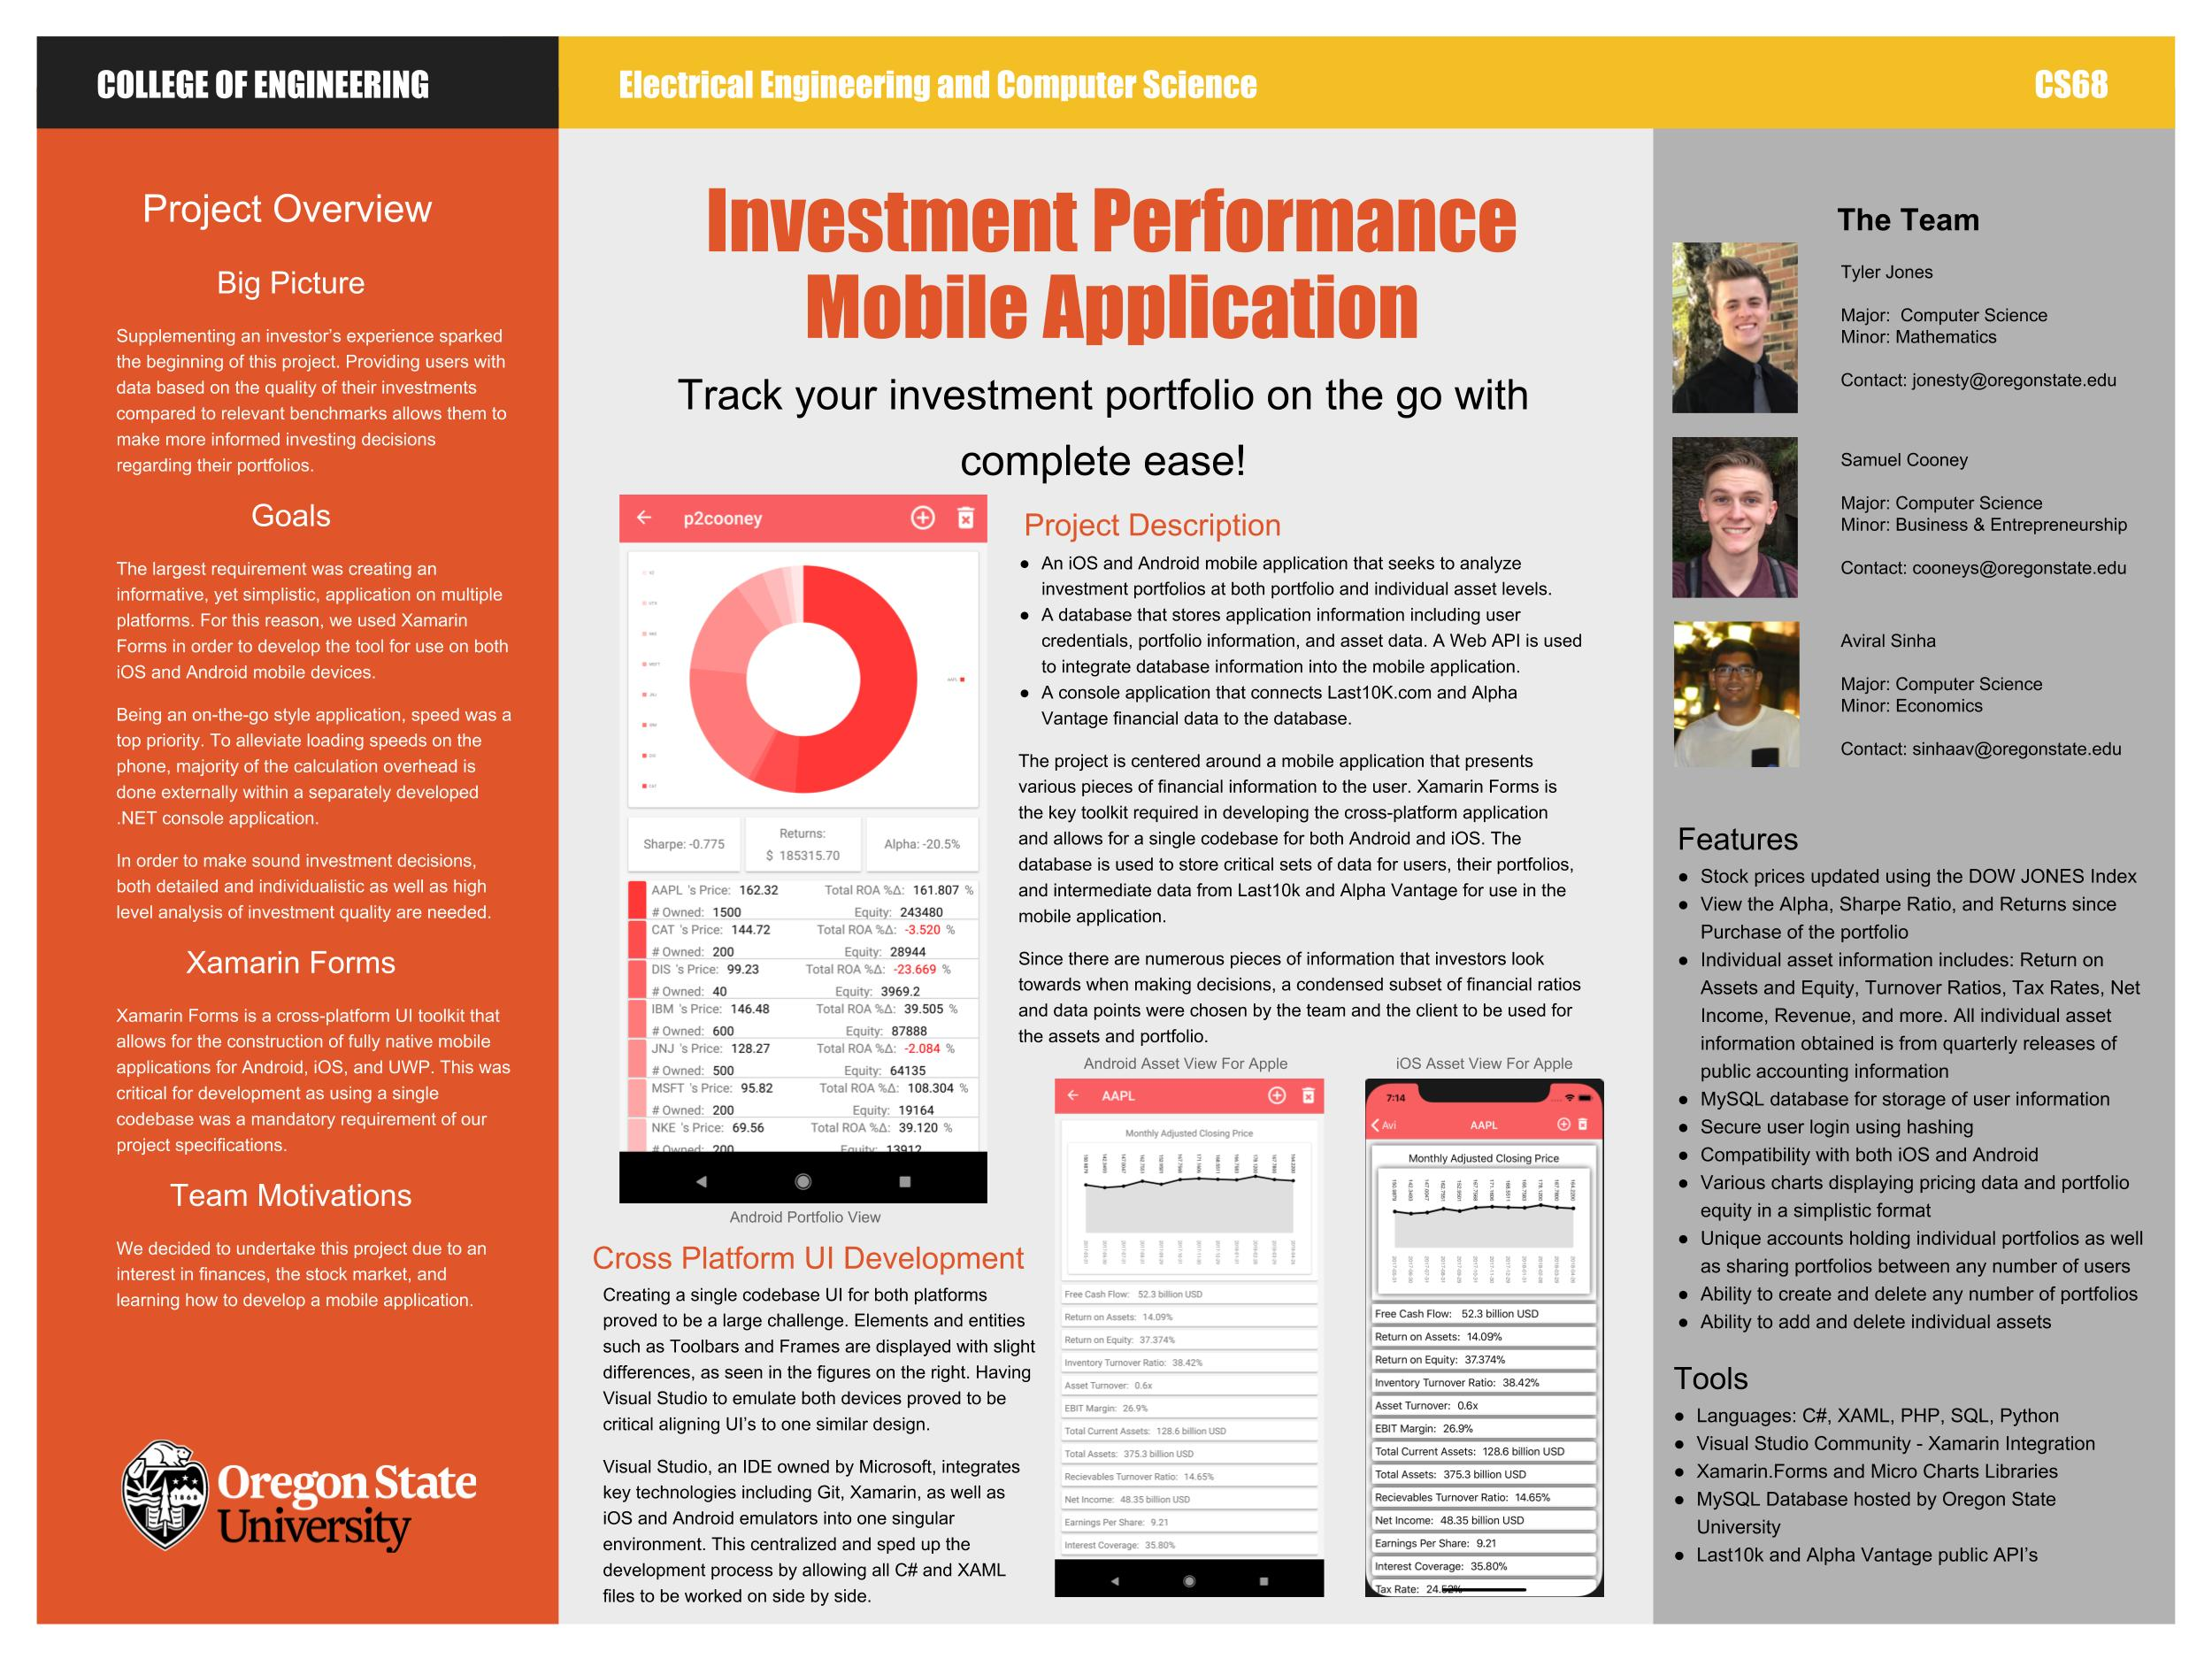
\includegraphics[scale=.25, angle=90]{poster.jpg}
    

\end{document}







